\documentclass[12pt]{article}

%-------------PACKAGES------------- 
\usepackage[margin=1in]{geometry} 
\usepackage{amsmath,amsthm,amssymb}
\usepackage{pgfplots}
\usepackage{float}
\usepackage{braket}
\usepackage{titling}
\usepackage{wrapfig}
\usepackage{tikz}
\usepackage{mwe}
\usepackage{enumitem}
\usepackage{mathtools}
\usepackage{scrextend}
\usepackage{listings}
\usepackage{color}
\usepackage{caption}
\usepackage{subcaption}
\usepackage{algorithm,algpseudocode}
\usetikzlibrary{shapes,arrows,chains}
\usetikzlibrary[calc]

%-------------FORMATTING-------------
\setlength{\droptitle}{-7.5em} 
\setlength{\parindent}{0pt}
\def\LW{\dimexpr.25\linewidth-.5em} 
\tikzstyle{line} = [draw, -latex']

%--------------COMMANDS--------------
\newcommand{\N}{\mathbb{N}}
\newcommand{\Z}{\mathbb{Z}}
\newcommand{\R}{\mathbb{R}}
\newcommand{\C}{\mathbb{C}}
%\renewcommand{\qedsymbol}{\filledbox}

\DeclarePairedDelimiter \abs{\lvert}{\rvert}%
\DeclarePairedDelimiter \babs{\bigg\lvert}{\bigg\rvert}%
\DeclarePairedDelimiter \norm{\lVert}{\rVert}%

%------------ENVIRONMENTS------------- 
\newenvironment{theorem}[2][]{\begin{trivlist}
		\item[{\bfseries #1}\hskip \labelsep {\bfseries #2.}]}{\end{trivlist}}
\newenvironment{lemma}[2][Lemma]{\begin{trivlist}
		\item[\hskip \labelsep {\bfseries #1}\hskip \labelsep {\bfseries #2.}]}{\end{trivlist}}
\newenvironment{exercise}[2][Exercise]{\begin{trivlist}
		\item[\hskip \labelsep {\bfseries #1}\hskip \labelsep {\bfseries #2.}]}{\end{trivlist}}
\newenvironment{reflection}[2][Reflection]{\begin{trivlist}
		\item[\hskip \labelsep {\bfseries #1}\hskip \labelsep {\bfseries #2.}]}{\end{trivlist}}
\newenvironment{proposition}[2][Proposition]{\begin{trivlist}
		\item[\hskip \labelsep {\bfseries #1}\hskip \labelsep {\bfseries #2.}]}{\end{trivlist}}
\newenvironment{corollary}[2][Corollary]{\begin{trivlist}
		\item[\hskip \labelsep {\bfseries #1}\hskip \labelsep {\bfseries #2.}]}{\end{trivlist}}
\newenvironment{definition}[2][]{\begin{trivlist}
		\item[{\bfseries #1}\hskip \labelsep {\bfseries #2.}]}{\end{trivlist}}
\theoremstyle{remark}
\newtheorem*{remark}{Remark}

%-------------CODE-STYLE------------
\definecolor{dkgreen}{rgb}{0,0.6,0}
\definecolor{gray}{rgb}{0.5,0.5,0.5}
\definecolor{mauve}{rgb}{0.58,0,0.82}
\lstset{frame=tb,
	language=C++,
	aboveskip=3mm,
	belowskip=3mm,
	showstringspaces=false,
	columns=flexible,
	basicstyle={\small\ttfamily},
	numbers=none,
	numberstyle=\tiny\color{gray},
	keywordstyle=\color{blue},
	commentstyle=\color{dkgreen},
	stringstyle=\color{mauve},
	breaklines=true,
	breakatwhitespace=true,
	tabsize=3
}

\tikzset{
	path image/.style={
		path picture={
			\node at (path picture bounding box.center) {
				\includegraphics[height=3cm]{example-image}};}},
	path tikzimage/.style={
		path picture={
			\node at (path picture bounding box.center)
			[circle, fill=blue!50, scale=2, text=yellow]{Bravo};}}
}

\lstset{
	morekeywords={end}
}

%------------------------------------ 
%---------START-OF-DOCUMENT----------
%------------------------------------
\begin{document}
	
	\title{Paper Summary}
	\author{David Miller \\ 
		CIS 5930: Social Network Mining} 
	
	\maketitle 
	
	\begin{figure}[H]{}
		\centering
		\vspace{-15pt}
		\hspace{-10pt}
		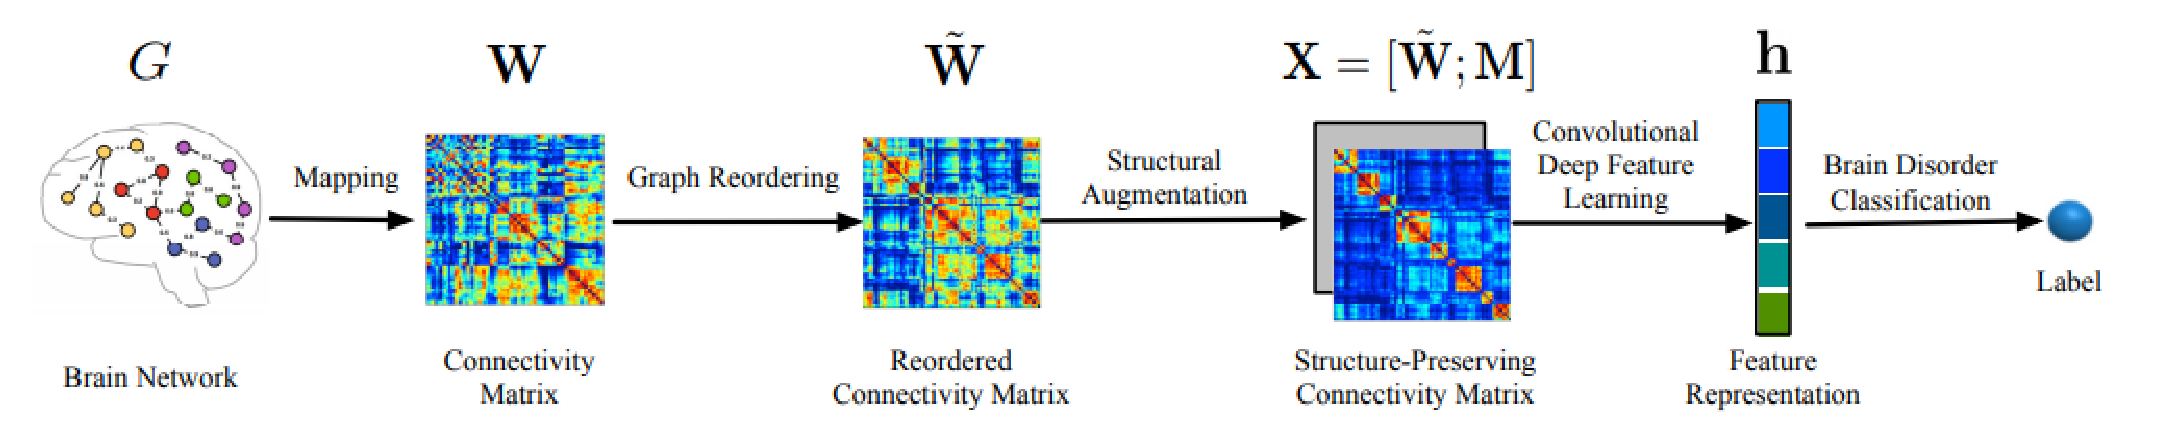
\includegraphics[height=3.25cm,width=1\textwidth]{fig1.eps}
		\caption{}
		\vspace{0pt}
	\end{figure} 
	
	\begin{wrapfigure}{r}{0.25\textwidth}
		\vspace{-15pt}
		\hspace{-20pt}
		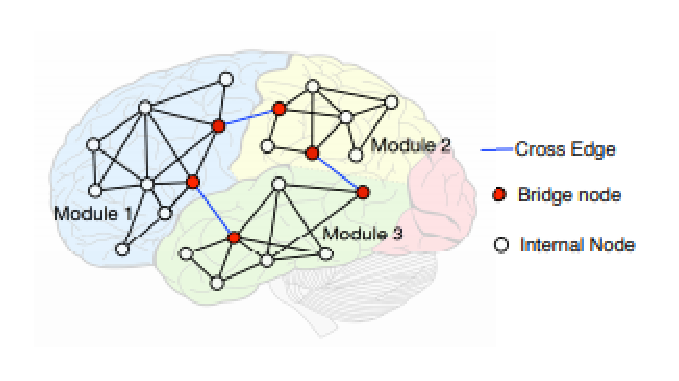
\includegraphics[height=3cm,width=0.31\textwidth]{fig2.eps}
		\caption{}
	\end{wrapfigure}
	
	Mining neurological data is a challenging data. The high non-linearity structure of the brain makes it very difficult for current algorithms to extract accurate representations, or modules, or connected networks. Figure 1 shows modules amongst lobe regions of the brain correctly represented. Amongst all the difficulties the method proposed in this paper, Structural Deep Brain Network (SDBN), attacks four main difficulties: high non-linearity found in underlying brain structure, noise produced from incorrect connection placements, structure preservation to maintain key roles among modules, and limited quantity and high dimensionality of data. Let $\mathcal{G} = \{G_1, \dots, G_N\}$ be a set of $N$ brain networks with weighted connectivity matrices $\mathcal{W} = \{W_i, \dots, W_N\}$, respectively. The goal of the algorithm is the accurately map $f:\mathcal{G} \rightarrow \mathcal{H}$, where $\mathcal{H}$ is a set of vector representations of the brain. The three main steps to the algorithm are:
	
	\begin{enumerate}
		\item \textbf{Graph Reordering:} Let $\boldsymbol{L}$ be the Laplacian matrix of the average connectivity matrix $\boldsymbol{\hat{W}}$. $K$-means clustering is applied to $\boldsymbol{L}$ to achieve $K$ modules $\mathcal{M} = \{M_1, \dots, M_K\}$ with $V = M_1 \cup \dots \cup M_K$ and $M_i \cap M_j = \emptyset$ for all $i, j$ such that $i \neq j$. From this the reordered connectivity matrix $\\boldsymbol{tilde{W}}$ for each brain network is produced.
		\item \textbf{Structural Augmentation:} A module identification $\boldsymbol{M}$ is used to encode the module structure information where 
		\begin{align*}
		m_{i,j} = 
		\begin{cases}
		k \quad \text{for} & v_i, v_j \in M_k, \, k = 1, \dots, K \\
		0 \quad \text{for} & i,j \not\in M_k , \, k = 1, \dots, K
		\end{cases}
		\end{align*}
		To matrix $\boldsymbol{M}$ is concatenated with the reordered connectivity matrix $\boldsymbol{\tilde{W}}$.
		\item \textbf{Unsupervised Learning Augmenting CNN:} The resulting connectivity matrices are fed into a CNN for feature representation. 
	\end{enumerate}
	
	The obvious future work of this algorithm would be implementation in hospital and physiological structures for early brain disorder detection. Another direction of future work would be generalizing the algorithm for connected networks that need to classify abnormalities, such as crime locations in huge cities. The last direction this paper should head in is scalability. There is no mention of scalability and it is pivotal for today's algorithm to be scalable. \\
	
	Three strengths I found with the paper are
	\begin{enumerate}
		\item The application of the SBDN network in the medical field can help lower money spent on healthcare through early detection. 
		\item The algorithm is built upon existing ideas (graph theory, machine learning, neural networks) making it easy to understand and adapt. 
		\item The SBDN algorithm lends itself well to problems with highly non-linear structure, subgroups, or modules, or networks, that can be used to identify the global network as "regular" or "irregular". 
	\end{enumerate} 
	\vspace{0.5cm}
	
	Three weaknesses I found with the paper are
	\begin{enumerate}
		\item There is no mention of scalability. Since there is no mention of the test bench used, I can not assume it can be done on a personal computer. 
		\item Although the accuracy from the algorithm is higher than existing ones, the overall accuracy does not seem high enough for professional use. 
		\item The data available for brain imaging networks is limited.
	\end{enumerate}
	\vspace{0.5cm}
	
	Questions for the reader
	\begin{enumerate}
		\item How exactly does the CNN work? It wasn't exactly clear how it worked as described in the paper. 
		\item How does the accuracy scale with an increase in samples?
	\end{enumerate}
	\vspace{0.5cm}
	
	\begin{thebibliography}{unsrt}
		\bibitem{paper}
		Shen Wang, Lifang He, Bokai Cao, Chun-Ta Lu, Philip S. Yu, Ann B. Ragin \emph{Structural Deep Brain Network Mining}, KDD’17, August 13-17, 2017, Halifax, NS, Canada.
	\end{thebibliography}
	
\end{document}\documentclass[12pt]{article}